Please draw the vector $u = \boldsymbol{B}v$, where $\boldsymbol{B}$ is

\begin{align*}
    \boldsymbol{B} = \begin{bmatrix}
    cos(30\degree) & -sin(30\degree) \\
    sin(30\degree) & cos(30\degree)
    \end{bmatrix}
\end{align*}

\begin{solution}
\begin{align*}
    \boldsymbol{Bv} = \begin{bmatrix}
    \frac{\sqrt{3}}{2} \\
    \frac{1}{2}
    \end{bmatrix}
\end{align*}

\begin{center}
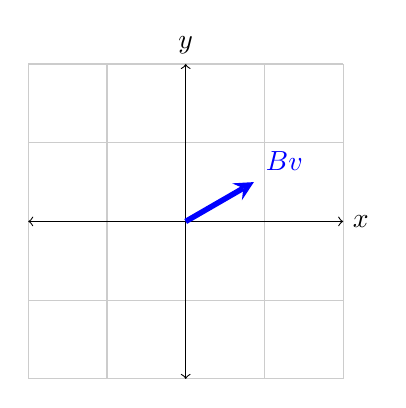
\begin{tikzpicture}
  \draw[thin,gray!40] (-2,-2) grid (2,2);
  \draw[<->] (-2,0)--(2,0) node[right]{$x$};
  \draw[<->] (0,-2)--(0,2) node[above]{$y$};
  \draw[line width=2pt,blue,-stealth](0,0)--(0.866,0.5) node[anchor=south west]{$\boldsymbol{Bv}$};
\end{tikzpicture}
\end{center}
\end{solution}